\section{Introduction}
\label{sec:introduction}
% Thesis introduction
% Prendi l'abstract della tesi fino a dove dice model simulation (incluso).
During pregnancy, the fetal airways are filled with a fluid known as
fetal lung fluid, which is essential for the development of
airways. Consequently, at birth, the respiratory system must expel
this fluid to allow aeration. Preterm infants may not be able to
adequately achieve lung aeration at birth autonomously. The
application of a positive pressure waveform at the airway opening can
support them. However, the best pressure strategy for promoting lung
aeration without damaging the fragile lung is still unknown. Model
simulation can help in the definition of such a strategy.


% Prendi 7 righe delle conclusioni
Anatomical morphometric models of the adult lung have been extensively
developed starting from the asymmetric model of Horsfield
(\cref{fig:albero_dicotomico_anatomical}). They were used in the
literature to enhance our understanding of pulmonary pathologies and
to guide treatments. In contrast, anatomical morphometric models of
the newborn lung are largely absent. It's not sufficient to simply
scale down models developed for adult lungs to fit newborn
lungs. Newborn lungs are not merely smaller versions of adult lungs;
they exhibit significant differences in morphometric characteristics,
airway wall structure, and tissue composition and properties. These
differences must be considered when developing or adapting
mathematical models to accurately represent the functioning of newborn
lungs.

%% Albero di Horsfield (Lutchen). SPOSTA IN INTRODUZIONE
\begin{figure}[H]\centering
  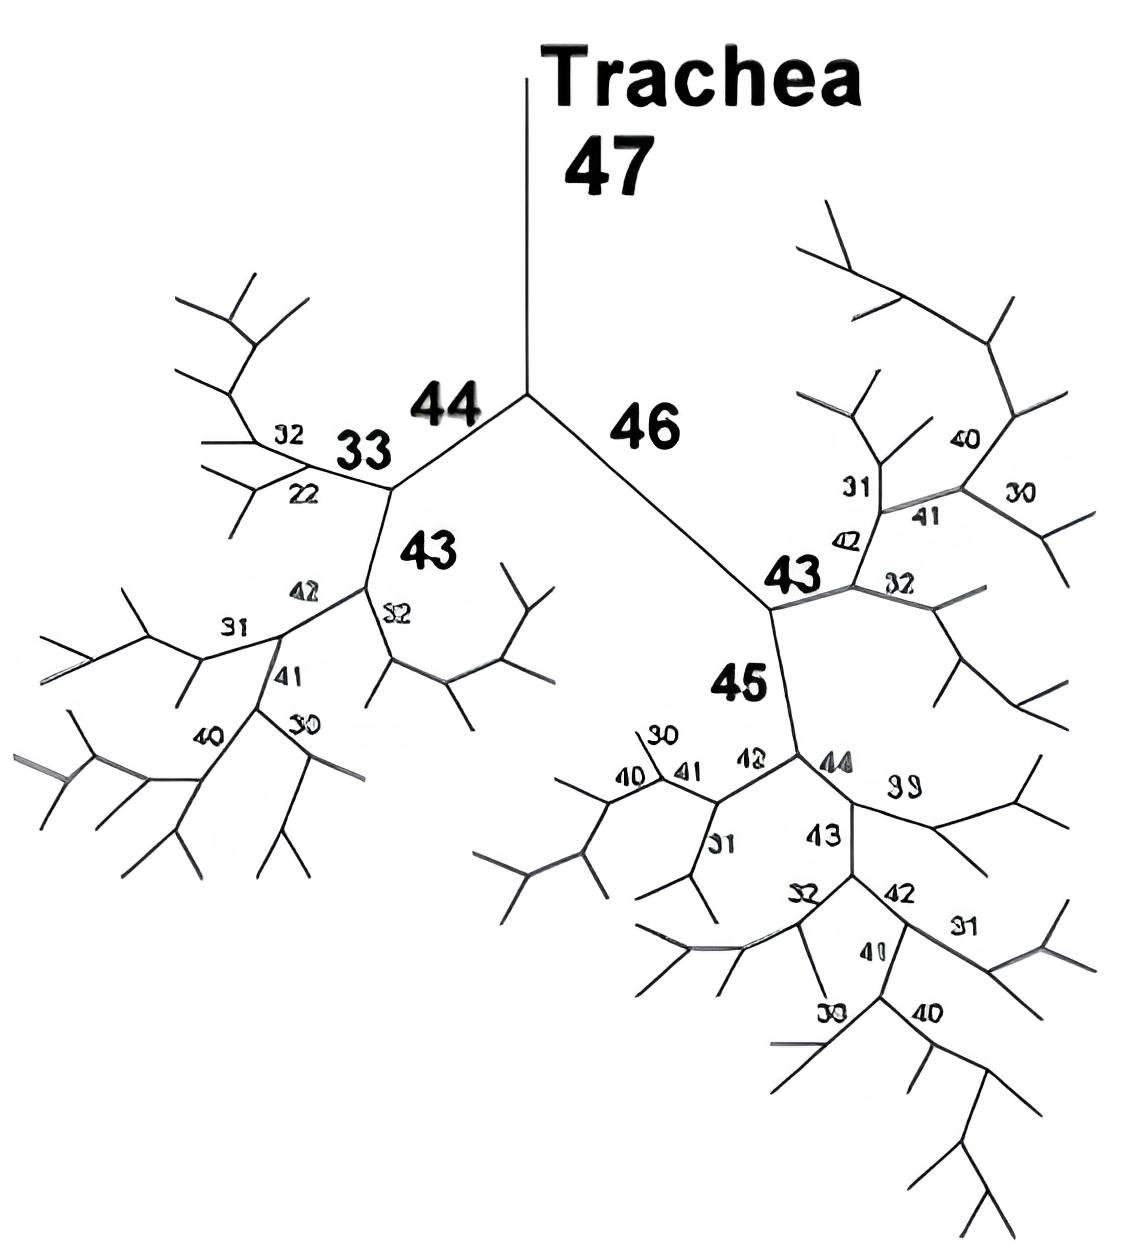
\includegraphics[width=.39\textwidth]{albero_dicotomico_best.png}
  \caption{The dichotomous bronchial tree.}
  \label{fig:albero_dicotomico_anatomical}
\end{figure}

% Prendi gli Aims
Aims of this projects are:
\begin{description}
\item Generate a model from neonatal CT scans to optimize the
  generation of airways, ensuring they adhere to the morphometric
  characteristics at various ages.
\item Develop an open-source mechanical model that allows for the
  simulation of mechanical properties along with fluid dynamics.
\end{description}

%%% Local Variables:
%%% mode: LaTeX
%%% TeX-master: "../Executive"
%%% End:
